\documentclass[12pt]{article}

% https://www.guitex.org/home/images/ArsTeXnica/AT015/drawing-ER-diagrams-with-TikZ.pdf
\usepackage{tikz-er2}
\usetikzlibrary{er, positioning}

\usepackage{pdfpages}
\pagestyle{empty}

\usepackage[a4paper, margin=0in]{geometry}

\pgfdeclarelayer{bg}    % declare background layer
\pgfsetlayers{bg,main}  % set the order of the layers (main is the standard layer)


\begin{document}
\includepdf[pagecommand={
	\begin{tikzpicture}[remember picture, overlay]
		\node at (16,-2.9) {100029};
		\node at (16,-3.8) {del Mazo};
		\node at (16,-4.6) {Federico};
	\end{tikzpicture}}]{Parcialito1-Enunciado}


\centering

\vspace*{\fill}
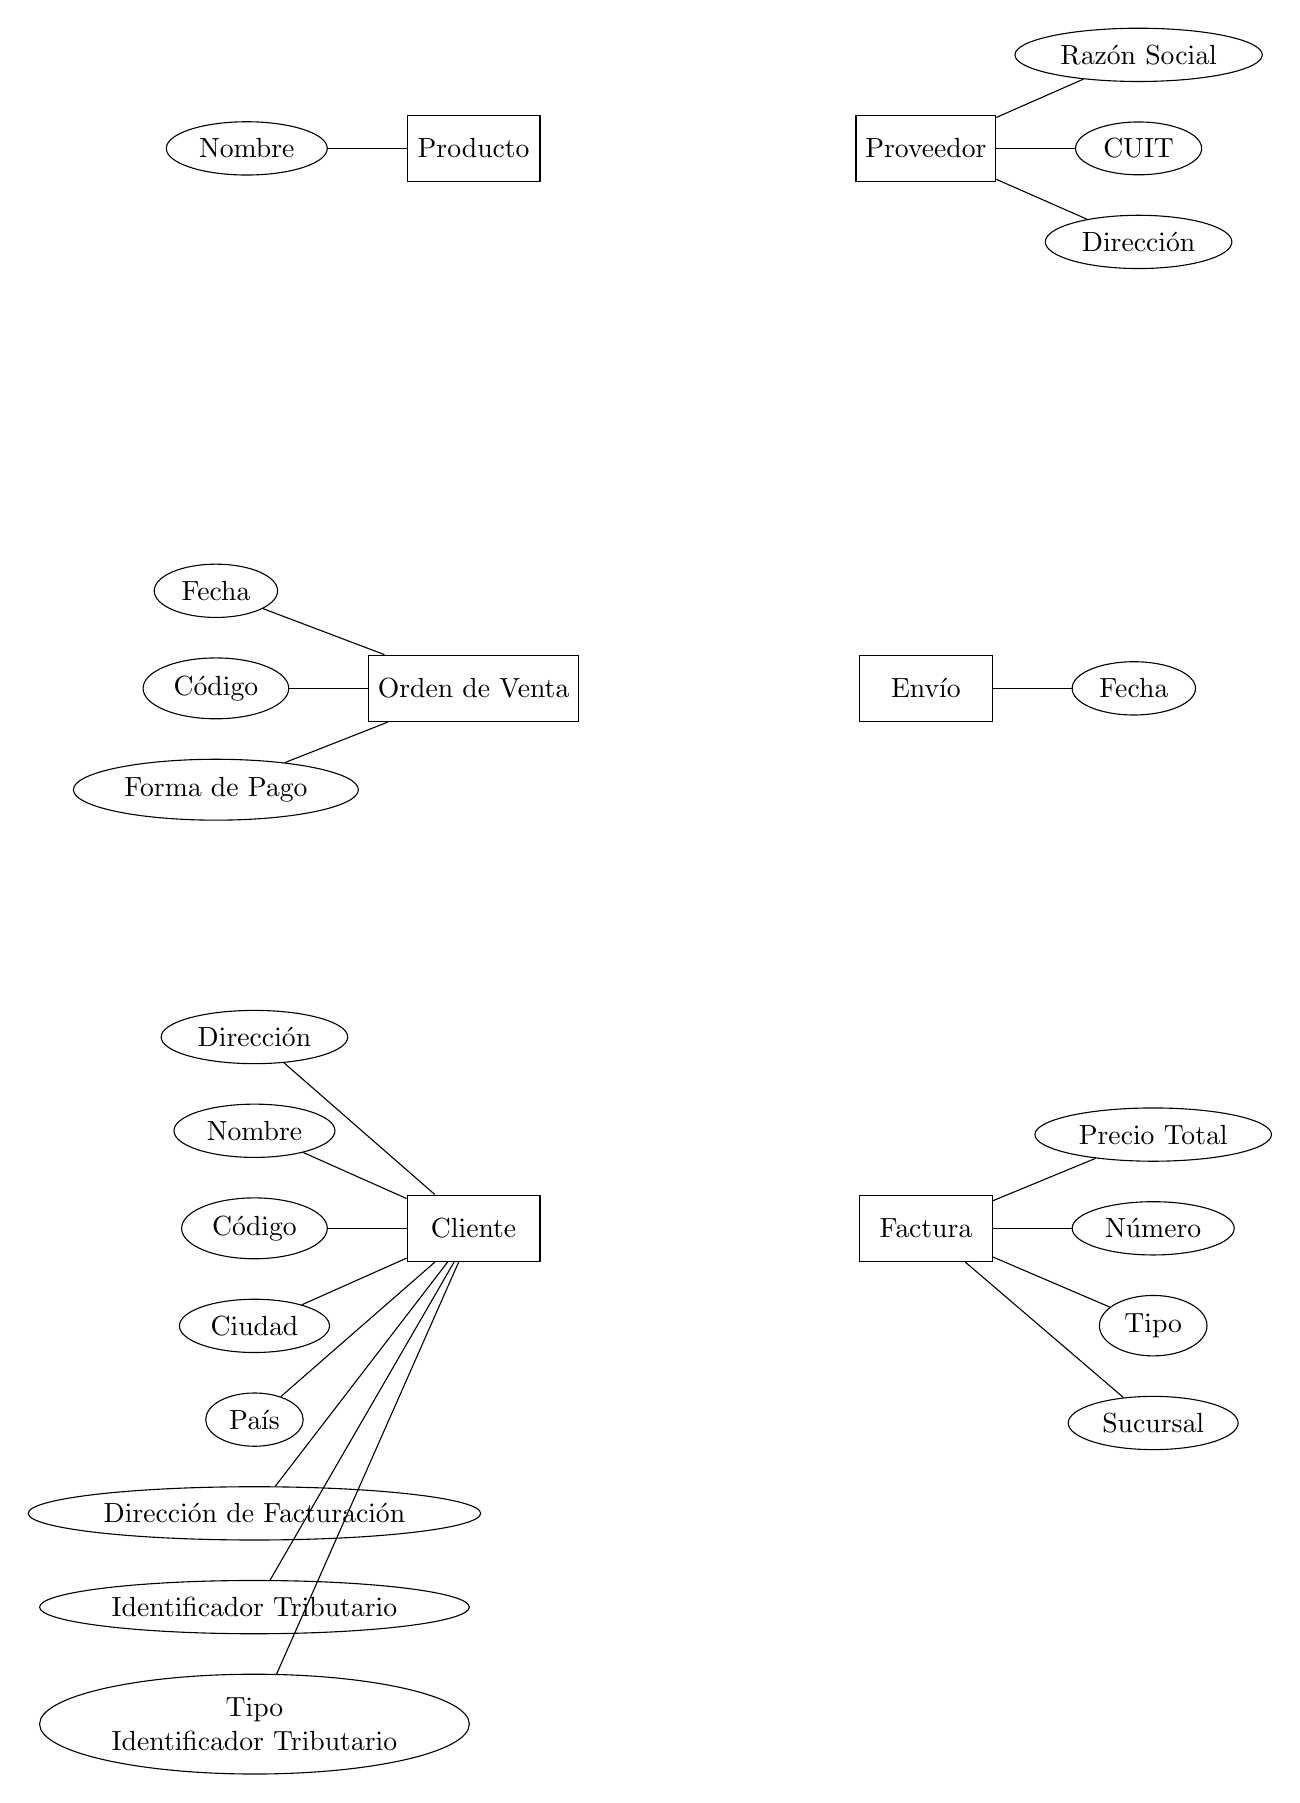
\begin{tikzpicture}[auto, node distance = 6cm and 1cm ]
  \node[entity] (producto) {Producto};
  \node[attribute] (producto_nombre) [left=of producto] {\key{Nombre}} edge (producto);

  \node[entity] (ordendeventa) [below=of producto] {Orden de Venta};
  \node[attribute] (ordendeventa_codigo) [left=of ordendeventa] {\key{Código}} edge (ordendeventa);
  \node[attribute] (ordendeventa_fecha) [above=0.5cm of ordendeventa_codigo] {Fecha} edge (ordendeventa);
  \node[attribute] (ordendeventa_formadepago) [below=0.5cm of ordendeventa_codigo] {Forma de Pago} edge (ordendeventa);

  \node[entity] (cliente) [below=of ordendeventa] {Cliente};
  \node[attribute] (cliente_codigo) [left=of cliente] {\key{Código}} edge (cliente);
  \node[attribute] (cliente_nombre) [above=0.5cm of cliente_codigo] {Nombre} edge (cliente);
  \node[attribute] (cliente_direccion) [above=0.5cm of cliente_nombre] {Dirección} edge (cliente);
  \node[attribute] (cliente_ciudad) [below=0.5cm of cliente_codigo] {Ciudad} edge (cliente);
  \node[attribute] (cliente_pais) [below=0.5cm of cliente_ciudad] {País} edge (cliente);
  \node[attribute] (cliente_direccionfacturacion) [below=0.5cm of cliente_pais] {Dirección de Facturación} edge (cliente);
  \node[attribute] (cliente_identificadortributario) [below=0.5cm of cliente_direccionfacturacion] {Identificador Tributario} edge (cliente);
  \node[attribute, align=center] (cliente_tipo_identificadortributario) [below=0.5cm of cliente_identificadortributario] {Tipo\\ Identificador Tributario} edge (cliente);

  \node[entity] (proveedor) [right=of producto, xshift=3cm] {Proveedor};
  \node[attribute] (proveedor_cuit) [right=of proveedor] {\key{CUIT}} edge (proveedor);
  \node[attribute] (proveedor_razon_social) [above=0.5cm of proveedor_cuit] {Razón Social} edge (proveedor);
  \node[attribute] (proveedor_direccion) [below=0.5cm of proveedor_cuit] {Dirección} edge (proveedor);

  \node[entity] (envio) [below=of proveedor] {Envío};
  \node[attribute] (envio_fecha) [right=of envio] {Fecha} edge (envio);

  \node[entity] (factura) [below=of envio] {Factura};
  \node[attribute] (factura_numero) [right=of factura] {\key{Número}} edge (factura);
  \node[attribute] (factura_precio) [above=0.5cm of factura_numero] {Precio Total} edge (factura);
  \node[attribute] (factura_tipo) [below=0.5cm of factura_numero] {Tipo} edge (factura);
  \node[attribute] (factura_sucursal) [below=0.5cm of factura_tipo] {Sucursal} edge (factura);

\end{tikzpicture}
\vspace{\fill}

\end{document}
